\documentclass{include/thesisclass}
% Main File - Based on thesisclass.cls
% Comments are mostly in English
% ------------------------------------------------------------------------------
% Further files in folder:
%  - include/cmds.tex (for macros and additional commands)
%  - include/kitlogo.pdf (for titlepage)
%  - lit.bib (bibtex bibliography database)
%  - include/titlepage.tex (for layout of titelpage)
% ------------------------------------------------------------------------------
% Useful Supplied Packages:
% amsmath, amssymb, mathtools, bbm, upgreek, nicefrac,
% siunitx, varioref, booktabs, graphicx, tikz, multicol





%% -------------------------
%% |    Thesis Settings    |
%% -------------------------
% english or ngerman (new german für neue deutsche Rechtschreibung statt german)
\SelectLanguage{english}
% details on this thesis
\newcommand{\thesisauthor}{Klara Fall}
\newcommand{\thesistopic}{Name des Themas auf Deutsch}
\newcommand{\thesisentopic}{Name of the Topic in English}
\newcommand{\thesislongtopic}{Very long and very detailed description of the very interesting thesis topic (only necessary for pdfsubject tag).}
\newcommand{\thesisinstitute}{Institut für Experimentelle Kernphysik}
\newcommand{\thesisreviewerone}{Prof. Dr. D. Cay}
\newcommand{\thesisreviewertwo}{Prof. Dr. E. Vil}
\newcommand{\thesisadvisorone}{} % to use: enter names and uncomment in titlepg
\newcommand{\thesisadvisortwo}{}
\newcommand{\thesistimestart}{01.04.2015} % on titlepage
\newcommand{\thesistimeend}{30.09.2015} % on titlepage
\newcommand{\thesistimehandin}{30.09.2015} % on second page 'preamble'
\newcommand{\thesispagehead}{Bachelor Thesis: \thesisentopic} % page heading





%% ---------------------
%% |    PDF - Setup    |
%% ---------------------
% This information will appear embed into the PDF file as meta data, but will 
% not be printed anywhere
\hypersetup
{
    pdfauthor={\thesisauthor},
    pdftitle={Bachelorarbeit: \thesistopic},
    pdfsubject={\thesislongtopic},
    pdfkeywords={kit,physik,bachelor,thesis,\thesisauthor}
}





%% --------------------------------------
%% |    Settings for Word Separation    |
%% --------------------------------------
% Help for separation:
% In German package the following hints are additionally available:
% "- = Additional separation
% "| = Suppress ligation and possible separation (e.g. Schaf"|fell)
% "~ = Hyphenation without separation (e.g. bergauf und "~ab)
% "= = Hyphenation with separation before and after
% "" = Separation without a hyphenation (e.g. und/""oder)

% Describe separation hints here:
\hyphenation
{
    über-nom-me-nen an-ge-ge-be-nen
    %Pro-to-koll-in-stan-zen
    %Ma-na-ge-ment  Netz-werk-ele-men-ten
    %Netz-werk Netz-werk-re-ser-vie-rung
    %Netz-werk-adap-ter Fein-ju-stier-ung
    %Da-ten-strom-spe-zi-fi-ka-tion Pa-ket-rumpf
    %Kon-troll-in-stanz
}





%% -----------------------
%% |    Main Document    |
%% -----------------------
\usepackage{lipsum} % for Lorem Ipsum text example
\begin{document}
    % Titlepage and ToC
    \FrontMatter

    % coordinates for background border
\newcommand{\diameter}{20}
\newcommand{\xone}{-15}
\newcommand{\xtwo}{160}
\newcommand{\yone}{15}
\newcommand{\ytwo}{-253}




\begin{titlepage}
    % background border
    \begin{tikzpicture}[overlay]
    \draw[color=gray]
            (\xone mm, \yone mm)
      -- (\xtwo mm, \yone mm)
    arc (90:0:\diameter pt)
      -- (\xtwo mm + \diameter pt , \ytwo mm)
        -- (\xone mm + \diameter pt , \ytwo mm)
    arc (270:180:\diameter pt)
        -- (\xone mm, \yone mm);
    \end{tikzpicture}



    % KIT image and sign for faculty of physics
    \begin{textblock}{10}[0,0](4.5,2.5)
        
\includegraphics[width=.25\textwidth]{include/kitlogo.pdf}
    \end{textblock}
    \changefont{phv}{m}{n}    % helvetica
    \begin{textblock}{10}[0,0](5.5,2.2)
        \begin{flushright}
            \Large FAKULTÄT FÜR PHYSIK\\%\thesisinstitute
        \end{flushright}
    \end{textblock}



    % horizontal line
    \begin{textblock}{10}[0,0](4.2,3.1)
        \begin{tikzpicture}[overlay]
        \draw[color=gray]
                (\xone mm + 5 mm, -12 mm)
          -- (\xtwo mm + \diameter pt - 5 mm, -12 mm);
        \end{tikzpicture}
    \end{textblock}



    % begin of text part
    \changefont{phv}{m}{n}    % helvetica
    \centering



    % thesis topic (en and ge)
    \vspace*{3cm}
    \Huge\thesistopic\\




    % author name and institute
    \vspace*{1cm}
    \Large Report\\by\\
    \vspace*{1cm}
    \huge\thesisauthor\\




    % possible frontimage - thanks to JabberWok
    % for publishing the img under GNU Document License
    \vspace*{1.5cm}
    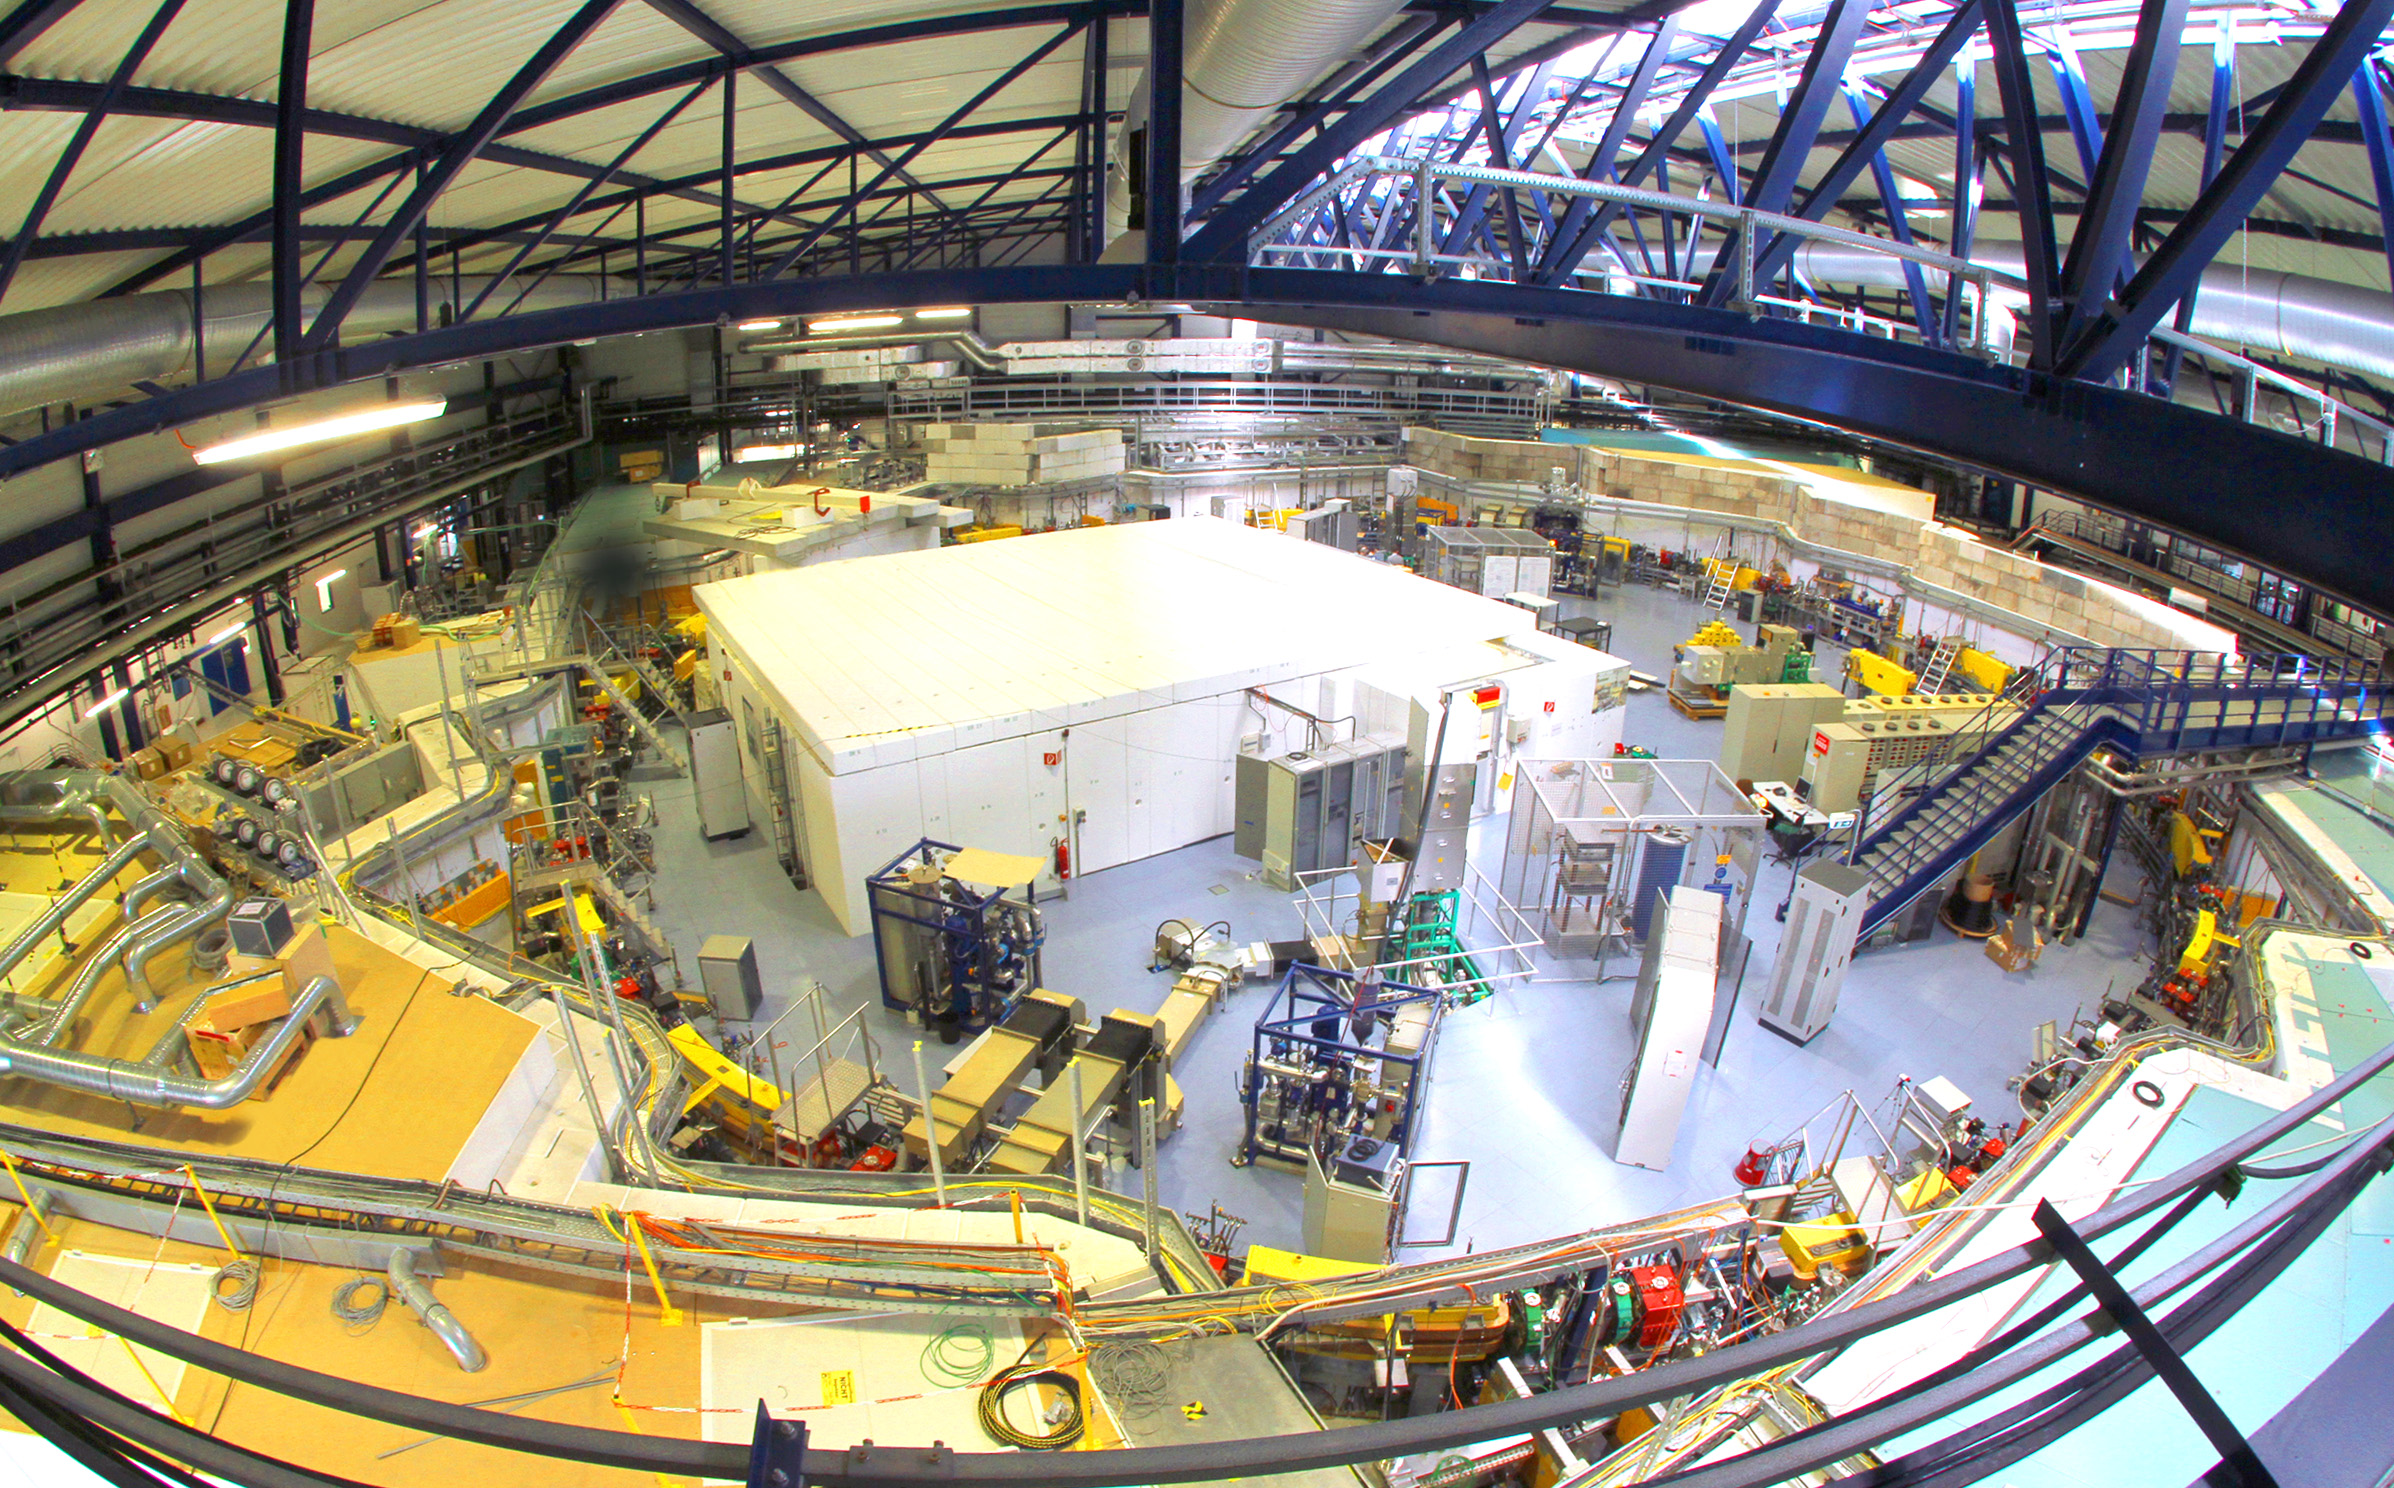
\includegraphics[scale=0.45]{./include/KIT_synchrotron_light_source_hall_view.jpg}\\
    \small{Reference: https://www.ibpt.kit.edu/kara.php}



    % examiners (Referenten)
%    \vspace*{1.5cm}
 %   \Large
  %  \begin{center}
   %     \begin{tabular}[ht]{l c l}
    %    \iflanguage{english}{Reviewer}{Referent}: 
     %       & \hfill & \thesisreviewerone\\
      %  \iflanguage{english}{Second Reviewer}{Korreferent}: 
       %     & \hfill & \thesisreviewertwo\\
        % uncomment if you want to provide info on your advisors
        %\iflanguage{english}{Advisor}{Betreuender Mitarbeiter}: 
        %    & \hfill & \thesisadvisorone\\
        %\iflanguage{english}{Second Advisor}{Zweiter betreuender Mitarbeiter}: 
        %    & \hfill & \thesisadvisortwo\\
       % \end{tabular}
    %\end{center}



    % working time
    \vspace{1.5cm}
    \begin{center}
        \large{{Time}: \thesistimestart }
    \end{center}



    % lowest text blocks concerning the KIT
    \begin{textblock}{10}[0,0](2,16.8)
        \tiny{KIT – Die Forschungsuniversität in der Helmholtz-Gemeinschaft}
    \end{textblock}
    \begin{textblock}{10}[0,0](10,16.75)
        \large{\textbf{www.kit.edu}}
    \end{textblock}
\end{titlepage}

    \chapter*{Erklärung zur Selbstständigkeit}
Ich versichere, dass ich diese Arbeit selbstständig verfasst habe und keine %
anderen als die angegebenen Quellen und Hilfsmittel benutzt habe, die %
wörtlich oder inhaltlich übernommenen Stellen als solche kenntlich gemacht und %
die Satzung des KIT zur Sicherung guter wissenschaftlicher Praxis in der %
gültigen Fassung vom 24.05.2018 beachtet habe.\\

\vspace{1cm}

\renewcommand{\arraystretch}{0} % for spacing in the tabular environment

\begin{flushright}
	\begin{tabular}{rr}
		Karlsruhe, den \thesistimehandin, & \hspace*{5cm}\\[0mm]
		\cline{2-2}\\[2mm]    % the last line has height 2mm due
		& \thesisauthor       % to \arraystretch=0
	\end{tabular}
\end{flushright}

\vfill

\begin{flushright}
	Als Prüfungsexemplar genehmigt von\\
	\vspace{1cm}
	\begin{tabular}{rr}
		Karlsruhe, den \thesistimehandin, & \hspace*{5cm}\\[0mm]
		\cline{2-2}\\[2mm]    % the last line has height 2mm due
		& \thesisreviewerone  % to \arraystretch=0
	\end{tabular}
\end{flushright}

\renewcommand{\arraystretch}{1}

\cleardoublepage


    \begingroup \let\clearpage\relax    % in order to avoid listoffigures and
    \tableofcontents                    % listoftables on new pages
    \listoffigures
    \listoftables
    \endgroup
    \cleardoublepage



    % Contents
    \MainMatter

    \chapter{Introduction}
    The computer exercises parts of the practicals focus on working with MADX, the CERN software to simulate beam dynamics and optimize beam optics in particle accelerators.
\section{Part I - Building your own FODO lattice and tracking}
As shown in listing \ref{lst:FODOcell} in a first step a single FODO cell is defined. Between two quadrupoles is a drift space \textit{dr} of length $D$. The quadrupoles are thin-lens elements defined over the \textit{multipole} command. The focussing quadrupole \textit{qf} has a strength of $1/f$, while the defocussing one \textit{qd} has $-1/f$, with $f$ being the focal length.\\
These elements are combined into a FODO cell \textit{fodo1} and the whole ring consists only of this one cell.\\
The particles are set to be electrons at an energy of $1.3\mathrm{\,GeV}$.

\begin{lstlisting}[caption=Defining the FODO cell,label={lst:FODOcell}]
D=1;
f=1;
qf: multipole, knl={0, 1/f};
dr: drift, l=D;
qd: multipole, knl={0, -1/f};
fodo1: line=(qf, dr, qd,dr);
ring: line=(fodo1);

beam, particle=electron, energy=1.3, sequence=ring;
use, sequence=ring;
\end{lstlisting}

In order to calculate the trajectories element by element through the thin-lens elements the \textit{track} command is used. It takes a relative momentum offset for the reference closed orbit (\textit{deltap}). The initial trajectory coordinates are given per trajectory/particle with one \textit{start} command. Here there particle has no momentum offset but starts slightly off center, so that the effects of the FODO cell can be seen.
The the actual tracking is triggered (\textit{run}) for the number of \textit{turns} given.\\
The results of the coordinate calculations per turn are saved in a table and with the \textit{plot} command plotted as phase space ellipses ($px$ over $x$ and $py$ over $y$).

\begin{lstlisting}[caption=Tracking,label={lst:tracking}]
track,  onepass, dump, deltap=0.001;
        start, x=3e-3, px=0, y=3e-3, py=0;
        run, turns=100;
endtrack;
plot, table=track, haxis=x, vaxis=px, particle=1, colour=1000, multiple, symbol=3, file=turns100d1f1;
plot, table=track, haxis=y, vaxis=py, particle=1, colour=1000, multiple, symbol=3, file=turns100d1f1;
\end{lstlisting}
Figure \ref{fig:ellipse} shows the phase space ellipse of $x$ and $y$ for $D=f=1$, a stable motion.
\begin{figure}
    \centering
    \includegraphics{}
    \caption{Caption}
    \label{fig:my_label}
\end{figure}

Whether a FODO cell is leading to a stable path can be seen from the stability criterion $|D/(2\cdot f)|<1$.

    \chapter{Theoretical Background}
    \section{Part IV - Working with KIT's storage ring KARA}
KARA is a $2.5\,\mathrm{GeV}$ electron storage ring. It's fed from a $90\,\mathrm{keV}$ electron gun, followed by a $53\,\mathrm{MeV}$ mictrotron and a last booster synchrotron up to $500\,\mathrm{MeV}$ before injection into KARA.
\par
In order to fill some current into KARA at first 
The magnetic fields in the bending and focusing elements are cycled to remove the magnetic hysteresis; they need to be raised from the low amplitude required at beam injection, to a maximum value, corresponding to peak beam energy and back again so as to be ready to accept the next pulse of injected beam.
The magnets have to be set to the current suitable for the injection energy as well as the RF frequency and amplitude.
After the injections magnets are turned on.
Then the trigger needs to be started to give a timing reference so as to synchronise different parts and power supplies of the kicker and the other magnets and the injection can start. 
Once enough current is in the ring the trigger and injection magnets can be stopped.\\
After it stopped the vertical orbit correction is turned on and the the energy ramp can be started. 
Reaching a certain energy also the horizontal orbit correction can be turned on.\\
The insertion devices (wiggler/undulator) are opened.
\par
The energy ramp...
\par

%++++++++++++++++++++++++++++++++++++++++++++++++++++++++++++++
\section{Part V - Network analyzer}
In this part a network analyzer is used to determine the properties of different devices.\\
For that it first has to be calibrated. According to the Open-Short-Load procedure both ports of the network analyzer are connected to the 'open' and then to the 'short' termination standards for calibration and a measurement is performed. In the first case, an open port, the signal will be fully reflected. For the short-circuited case the also fully reflected signal will have a $\pi$ phase shift.
\par
Following, for two different coaxial cables, RG58 and RG59, with characteristic impedances of $Z=\sqrt{\frac{L}{C}}=50\,\mathrm{\Omega}$ and $75\,\mathrm{\Omega}$ respectively, the attenuation and reflection  for $50$ to $1500\,\mathrm{MHz}$ are investigated.
The reflection coefficient is $r=\left|\frac{\text{Reflected power}}{\text{Incident power}}\right|$ and thus the return loss is $10\cdot\log(r)$ in dB. Analogously for the transmission coefficient $t=\left|\frac{\text{Transmitted power}}{\text{Incident power}}\right|$.\\
Figures \ref{fig:refl} and \ref{fig:trans} show the reflection and attenuation for both cables.
\begin{figure}[tbp]
\begin{minipage}{0.49\textwidth}
        \centering
        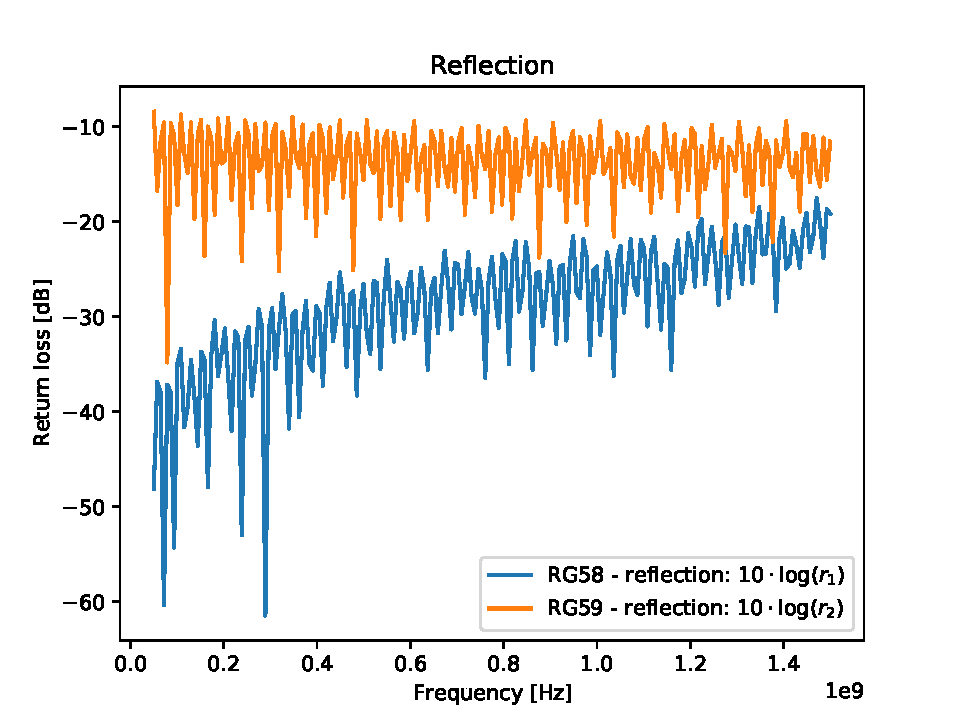
\includegraphics[width=1.1\linewidth]{../../part5/reflection.pdf}
        \caption{Reflection of RG58 and 59}
        \label{fig:refl}
    \end{minipage}\hfill
    \begin{minipage}{0.49\textwidth}
        \centering
        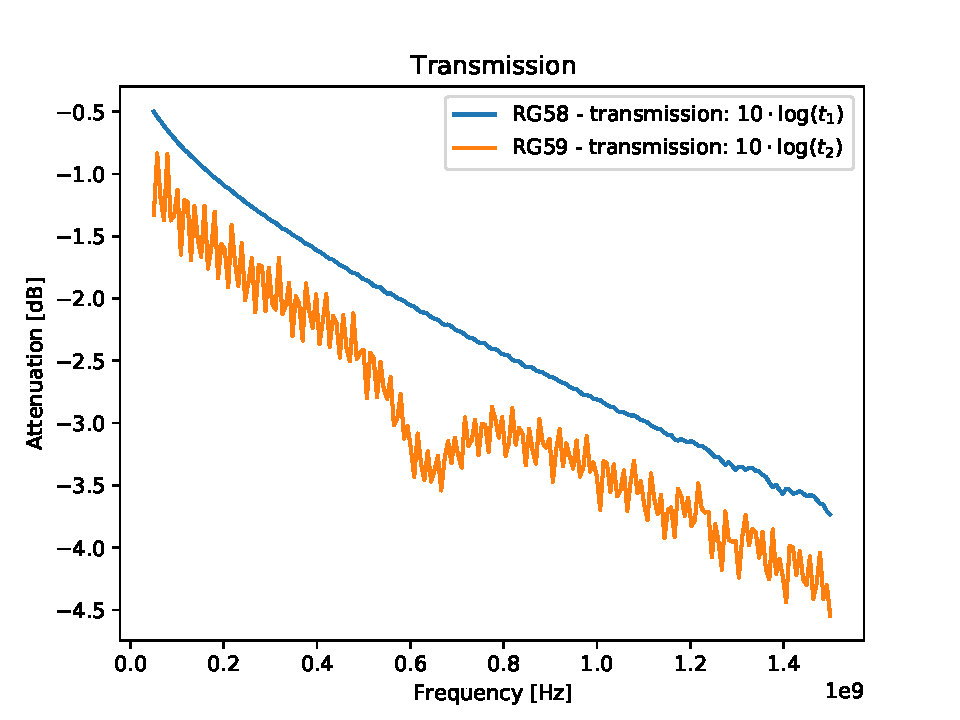
\includegraphics[width=1.1\linewidth]{../../part5/transmission.pdf}
        \caption{Attenuation of RG58 and 59}
        \label{fig:trans}
    \end{minipage}
\end{figure}
For both cables the transmission decreases for higher frequencies. The reflection is rather stable for the RG59 while it increases for the RG48 with higher frequencies.\\
Comparing the amplitudes of the signals, the RG58 has a higher transmission and but also higher reflection as the RG59, which is due to the lower wave impedance of the RG58.
\par
A further investigated device is a \textit{circulator} with a frequency range of $300$ to $450\,\mathrm{MHz}$. It has 3 ports and on all of them as well as between each pair the transmission and reflections will be determined. Thus for this device with 3 ports, the S-matrix has the dimensions $3\times3$:
$$S_{\mathrm{Circulator}}=\begin{pmatrix}-20.8&-20.5&-0.81\\-0.80&-21.4&-18.6\\-19.0&-0.79&-22.9\end{pmatrix}\,.$$
This matrix shows that the the incoming power can be transmitted almost without attenuation fro port 1 to 2, 2 to 3 and 3 to 1. It thus passed around to in a 'circle'. All other connections and directions are strongly ($\sim -20\,\mathrm{dB}$) attenuated.\\
When performing this measurement it is necessary to properly terminate the ports not connected to the network analyzer. Otherwise there will be reflection on the open ports interfering with the measurement as they are not suppressed at least in one direction. Without the termination there is significant transmission also in the other direction of the circle.\\
Input can be any of the ports while the following port in the circel should then serve as an output.\\
Circulators are for example used to connect a klystron to the RF-cavity to feed it with the high-frequency signal. A circulator protects in this case the klystron from the power reflected back from the cavity.
\par
As a last device a \textit{directional coupler} is characterised. It also has 3 ports and its S-matrix has the following form:
$$S_{\mathrm{dir.\,coupler}}=\begin{pmatrix}-29.0&-0.08&-30.0\\-0.08&-34.0&-55.0\\-30.1&-55.0&-23.0\end{pmatrix}\,.$$
From the matrix one can deduce that a directional coupler transmits in both direction from port 1 (the input port) to 2 (the transmitted port) and back ($-0.08\,\mathrm{dB}$). 
The third port, the coupled port, can be used as a port to connect a measurement device, which only receives a by 30\,dB attenuated signal from the input and is thus protected from the main power to be transmitted. 
%++++++++++++++++++++++++++++++++++++++++++++++++++++++++++++++
\section{Part VI - Cavity}
Finally a pillbox-like cavity will be analysed. With different cavity designs the bandwidth, coupling of the waves to the particles and central frequency can vary.\\
The setup consist of the cylindrical cavity (outer diameter $d=100.75\,\mathrm{mm}$, length $l=69.69\,\mathrm{mm}$ and a material thickness of $4\,\mathrm{mm}$) with a hole on each side with a fishing line passing through the cavity. The line can be moved with a small stepper motor so that a dielectric bead threaded on this line can be pulled through the cavity with a certain step size and total distance.\\
The cavity also has two screws which can be screwed into the lateral surface to change its geometry and thus the cavity's resonance frequency.
\par
With the aid of a network analyzer and the connected LabView
program the reflection coefficient is measured and the resonance frequency $f_0$ and quality factor $Q=f_0/B$ are determined. 
The cavity will reflect the incident power back as long as the frequency is not hitting the resonance. 
In case of the incident signal having the cavity's resonance frequency, the power will be absorbed into the cavity.\\
$B=f_2-f_1$ is the bandwidth where $f_2$ and $f_1$ are the upper and lower $-3\,\mathrm{dB}$ cutoff frequency (half-power point) respectively.
These are $$f_2=2.741100\,\mathrm{GHz}\text{ and }f_1=2.739573\,\mathrm{GHz}\,$$
and so $$B=1.527\,\mathrm{MHz}\,.$$
As the resonance peak is not symmetrical around the maximum the geometric mean rather than the arithmetic mean of the cutoff frequencies is used to calculate the resonance frequency. It becomes $$f_0=2.740336\,\mathrm{GHz}$$
and so the quality factor is
$$Q=1794.59\,.$$
\par
The electrical field inside the cavity is measured with the help of the differently sized dielectric beads pulled through the cavity on the fishing thread.\\
Due to the bead the resonance frequency changes and the change is related to the electrical field at a certain position $z$ over
$$E(z)\propto\sqrt{\frac{\Delta f_0(z)}{f_0}\cdot\frac{1}{V_{\text{bead}}}}\,.$$
    \chapter{Experimental Investigations}
    \lipsum[1-10]


    \emptychapter[3]{ROOT Routines}     % usage: \emptychapter[page displayed 
                                        %        in toc]{name of the chapter}



    \chapter{Conclusions}
    \lipsum[1-5]


    % appendix for more or less interesting calculations
    \Appendix
    \chapter*{\appendixname} \addcontentsline{toc}{chapter}{\appendixname}
    % to make the appendix appear in ToC without number. \appendixname = 
    % Appendix or Anhang (depending on chosen language)
    \section{First Appendix Section}
Wonderful Appendix!

\lipsum[1-5]
 %\cleardoublepage



    % Bibliography
    \TheBibliography

    % BIBTEX
    % use if you want citations to appear even if they are not referenced to: 
    % \nocite{*} or maybe \nocite{Kon64,And59} for specific entries
    %\nocite{*}
    \bibliographystyle{babalpha}
    \bibliography{lit.bib}

    % THEBIBLIOGRAPHY
    %\begin{thebibliography}{000}
    %    \bibitem{ident}Entry into Bibliography.
    %\end{thebibliography}
\end{document}
